\documentclass[11pt, oneside]{amsart}
\usepackage{geometry}
\geometry{letterpaper}
\usepackage[francais]{babel}
\usepackage[utf8]{inputenc}
\usepackage{graphicx}
\usepackage{float}
\usepackage{etex,mathtools}
\usepackage{amssymb}
\usepackage{enumitem}
\usepackage{amsmath}
\usepackage{caption}
\usepackage{listings}
\usepackage{array}

\graphicspath{{images/}}

\title[]{Preliminary report, PGM}
\author[1]{Louis Thiry}
\author[2]{Thomas Kerdreux}
\author[3]{Nicolas Jouvin}

\begin{document}

\maketitle

\section{Understanding of the paper}

This paper presents an algorithm to learn non linear stationnary dynamics of a system.

The system can be viewed as a graphical model :

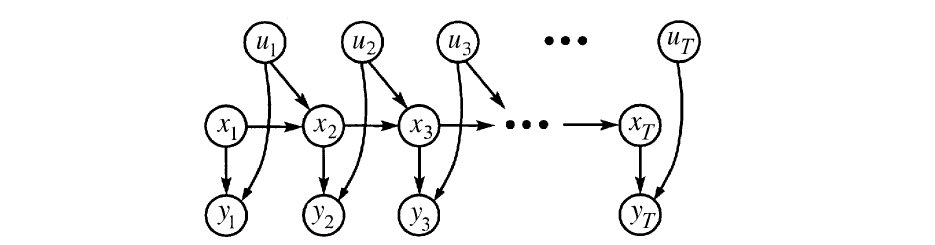
\includegraphics[width=14cm]{screenshot_graphical_model.PNG}
\captionof{figure}{Graphical model of our system.}

The dynamics of the system can be written in general as :
\begin{align*}
  x_{k+1} &= f(x_k, u_k) + w_k\\
  y_k &= g(x_k, u_k) + v_k\\
\end{align*}
$f$  and  $g$  are non linear function that we want to learn.
$w_k$ and  $v_k$ are zero mean Gaussian noise processes.

We assume that we have incomplete observations :
\begin{itemize}
  \item the inputs $u_k$ and outputs $y_k$, $k \in [1:T]$ are observed.
  \item the hidden states $x_k$ are unknown
\end{itemize}

So to learn the non linear dynamics of the system, we need to infer the hidden states.
Thus, the algorithm presented in this paper constist in an EM algortithm:
\begin{itemize}
  \item \textbf{E-step.}
    In the E-step, we need to do inference on the hidden states $x_k$.
    Since this problem is in general complex for our non linear equation, we linearize them around $\hat{x}_k$, the mean of the density $p(x_k | y_1, ... , y_k)$ :
    \begin{align*}
      x_{k+1} &= f(\hat{x}_k, u_k) + A_{\hat{x}_k} (x - x_k) + w_k\\
      y_k &= g(\hat{x}_k, u_k) + C_{\hat{x}_k} (x - x_k) + v_k\\
    \end{align*}
    With this simplification, we can apply an Extended Kalman Smoothing to perform et E-step and get the conditionnal probabilities on the hidden states :
    \begin{align*}
      P(x_k |u_1, ..., u_T, y_1, ... , y_T),& k \in [1,T]\\
      P(x_{k+1}, x_k |u_1, ..., u_T, y_1, ... , y_T),& k \in [1,T-1]\\
    \end{align*}
  \item \textbf{M-step.}
    In the M-step, we want to learn the parameter of the functions $f$ and $g$.
    In the paper, these function are assumed to be of the form:
    \begin{align*}
      f(x,u) &= \sum_{i=1}^I h_i \rho_i(x) + Ax + Bu + b + w\\
      \rho_i(x) &= \frac{1}{(2\pi)^{d/2}|S_i|^{1/2}} exp\left(-\frac{1}{2}(x-c_i)^TS_i^{-1}(x-c_i)\right)\\
    \end{align*}
    $w$ is a zero-mean Gaussian noise variable with covariance $Q$.
    The centers $c_i$ and width $S_i$ of the $\rho_i$ (called radial basis functions) are supposed to be known.
    With these assuption, the value of the parameters $\theta = \left( h_1, ..., h_I, A, B, b\right)$ and $Q$ can be expressed in close form.
\end{itemize}

The algorithm is tested first on generated data.
% commentaire sur la forme bien particulière de ces fonction : douille

\section{Planned implementations}

1. Kalman filter


\end{document}
